% file: example.tex
%
% Use:
% 	$ pdflatex -shell-escape <filename.tex>
% to generate a png image.

\documentclass[11pt,tikz,border=1,convert={outfile=\jobname.png}]{standalone}
\usetikzlibrary{calc,positioning,arrows.meta,shadows}

\begin{document}
  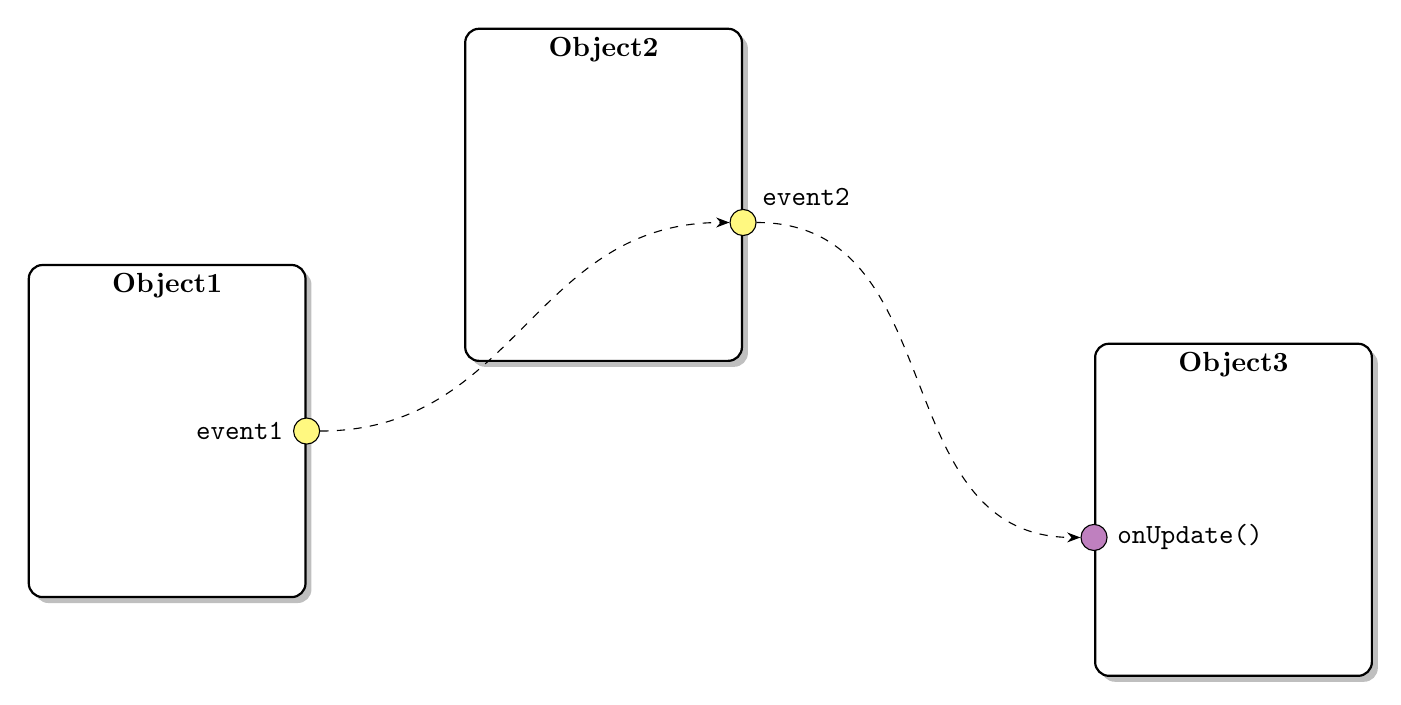
\begin{tikzpicture}[
    object/.style={thick,fill=white,rectangle,rounded corners=5pt,draw,minimum width=100pt,minimum height=120pt,drop shadow},
    token/.style={circle,draw,fill=yellow!50,minimum size=6pt},
    binding/.style={circle,draw,fill=violet!50,minimum size=6pt}
    ]

  \node(subject) [object] {};
  \node(subjectName) [below] at (subject.north) {\bf Object1};
  \node(event1) [token] at (subject.east) {};

  \node(observer1) [right=2cm of subject,yshift=3cm,object] {};
  \node(observer1Name) [below] at (observer1.north) {\bf Object2};
  \node(event2) [token,yshift=-10pt] at (observer1.east) {};

  \node(observer2) [right=10cm of subject,yshift=-1cm,object] {};
  \node(observer2Name) [below] at (observer2.north) {\bf Object3};
  \node(method2) [binding,yshift=-10pt] at (observer2.west) {};

  \coordinate(a) at ($(event1.east)+(25mm,0)$);
  \coordinate(b) at ($(event2.west)-(25mm,0)$);
  \coordinate(c) at ($(event2.east)+(25mm,0)$);
  \coordinate(d) at ($(method2.west)-(25mm,0)$);

  \draw[->,dashed,-{Stealth}] (event1) .. controls (a) and (b) .. (event2);
  \draw[->,dashed,-{Stealth}] (event2) .. controls (c) and (d) .. (method2);

  \node [left] at (event1.west) {\ttfamily event1};
  \node [right,yshift=2mm] at (event2.north east) {\ttfamily event2};
  \node [right] at (method2.east) {\ttfamily onUpdate()};

  \end{tikzpicture}
\end{document}
